\documentclass[12pt]{article}

\usepackage[margin=1in]{geometry} % 1-inch margins
\usepackage{times}                % Times (Times New Roman-like) font
\usepackage{fancyhdr}             % For custom headers/footers
\usepackage{setspace}             % For spacing
\usepackage{titlesec}             % For section formatting
\usepackage{enumitem}            % For list alignment
\usepackage{graphicx}             % For including images

\pagestyle{fancy}
\fancyhf{} % Clear default header and footer

% Header on the right side
\fancyhead[R]{Ultrasound Nerve Imaging And Clinical Decision Support System}

% Footer on the left side
\fancyfoot[L]{Pillai HOC College of Engineering \& Technology, Rasayani}
\fancyfoot[R]{\thepage} % Ensure page number is displayed on the right footer

% Horizontal lines in header & footer
\renewcommand{\headrulewidth}{0.4pt} 
\renewcommand{\footrulewidth}{0.4pt} 

% Set the page number to start from 14
\setcounter{page}{21}

\begin{document}

\vspace*{\fill}
\begin{center}
    {\Large \bf Chapter 4} \\[1em] % Line break with extra space (1em)
    {\Large \bf Plan of Project}
\end{center}
\vspace*{\fill}

\newpage

\vspace{15pt} % Adds space

% Set section counter to 3 so that it starts from 4
\setcounter{section}{4}

\newpage

% SUBSECTION 4.1: Methodology
\subsection{Methodology}

\vspace{10pt}

\noindent The methodology for the Ultrasound Nerve Imaging and Clinical Decision Support System combines deep learning-driven image analysis with a comprehensive web-based platform to deliver accurate disease diagnosis and actionable clinical guidance. The process initiates with the curation of ultrasound image datasets spanning thyroid disorders, breast cancer, kidney stones, and liver abnormalities, sourced from medical repositories and partnerships with healthcare institutions. These images undergo preprocessing steps such as augmentation to enhance variability and normalization to standardize pixel intensities, ensuring robustness across diverse imaging conditions. The data is partitioned into training, validation, and testing sets, with annotations for segmentation tasks focusing on regions of interest and classification labels derived from clinical diagnoses. Model development employs a dual architecture integrating convolutional neural networks for precise segmentation of anatomical structures or abnormalities and YOLOv11 for efficient multi-disease classification. The CNN-based segmentation model localizes disease-specific regions, while YOLOv11 leverages its single-pass detection framework to classify diseases rapidly without compromising accuracy, optimized via transfer learning and adjusted anchor boxes tailored to ultrasound lesion dimensions. The web platform, built using modern frameworks for backend and frontend operations, allows users to upload ultrasound images for real-time processing. Upon detection, the system generates a diagnostic report detailing the identified disease, confidence levels, and severity. Post-diagnosis, the platform dynamically provides clinical support by recommending medically validated next steps, such as follow-up tests or specialist consultations, and curates a list of experienced doctors filtered by expertise, patient reviews, and geographic proximity, alongside their contact details and hospital affiliations. Diet plans, designed in collaboration with nutritionists, are tailored to the diagnosed condition, specifying beneficial foods, restrictions, and meal schedules. Educational resources include simplified explanations of complex medical terms and curated YouTube content on disease management, yoga, or exercises, fetched via APIs to ensure relevance. System validation involves rigorous evaluation of segmentation accuracy using metrics like Dice coefficient and classification performance via F1-scores, tested across diverse demographics to ensure generalizability. Clinical recommendations are validated by physicians to align with established guidelines, while the platform prioritizes data security through encryption and transparency via explainable AI insights. By unifying AI-driven diagnostics with holistic post-diagnosis care, the methodology bridges the gap between imaging analysis and patient-centric healthcare, enabling timely interventions and informed decision-making for users.
\vspace{5pt}

\vspace{10pt}

\newpage

% SUBSECTION 4.2: Project Plan (Gantt Chart)
\subsection{Project Plan (Gantt Chart)}

\vspace{10pt}

\renewcommand{\thefigure}{4.2.\arabic{figure}}
\setcounter{figure}{0} % Reset counter for numbering
The development of this project follows a structured timeline represented in the Gantt Chart. The timeline includes key phases such as data collection, preprocessing, model development, testing, and system deployment. gantt chart for the Ultrasound Nerve Imaging and Clinical Decision Support System visually represents the project's timeline, tasks, and dependencies. It outlines key phases such as requirement analysis, dataset collection, model training (CNN and YOLOv11), system development, integration of clinical support features, testing, deployment, and user feedback evaluation. Each phase is allocated a specific time frame, ensuring efficient progress tracking. Milestones such as successful disease detection, report generation, and clinical recommendation implementation mark critical achievements.

\centering
\hspace{}
\begin{tabular}{|c|p{7cm}|c|c|c|}
\hline
\textbf{Sr. No.} & \textbf{Task Name} & \textbf{Start} & \textbf{Finish} & \textbf{Duration (days)} \\
\hline
1  & Topic Discussion & 12-07-2024 & 01-08-2024 & 15 \\
\hline
2  & Topic Selection & 02-08-2024 & 22-08-2024 & 15 \\
\hline
3  & Topic Research & 23-08-2024 & 12-09-2024 & 15 \\
\hline
4  & Design Module for Ultrasound Image & 13-09-2024 & 16-09-2024 & 2 \\
\hline
5  & Design Module for Disease Segmentation & 17-09-2024 & 30-09-2024 & 10 \\
\hline
6  & Design Module for Identify Nerve & 01-10-2024 & 09-10-2024 & 7 \\
\hline
7  & Design Module for Disease Detection & 10-10-2024 & 22-10-2024 & 9 \\
\hline
8  & Design Module for Health Report & 23-10-2024 & 01-01-2025 & 51 \\
\hline
9  & Implementation for Ultrasound Image & 16-09-2024 & 20-09-2024 & 5 \\
\hline
10 & Testing for Ultrasound Image & 20-09-2024 & 23-09-2024 & 2 \\
\hline
11 & Implementation for Disease Segmentation & 26-09-2024 & 04-10-2024 & 7 \\
\hline
12 & Testing for Disease Segmentation & 07-10-2024 & 15-10-2024 & 7 \\
\hline
13 & Implementation for Identify Nerve & 28-10-2024 & 14-11-2024 & 14 \\
\hline
14 & Testing for Identify Nerve & 15-11-2024 & 21-11-2024 & 5 \\
\hline
15 & Implementation for Disease Detection & 18-10-2024 & 28-11-2024 & 30 \\
\hline
16 & Testing for Disease Segmentation & 27-11-2024 & 02-12-2024 & 6 \\
\hline
17 & Implementation for Health Report & 20-12-2024 & 06-02-2025 & 35 \\
\hline
18 & Testing for Health Report & 06-02-2025 & 12-02-2025 & 6 \\
\hline
19 & Integration of All Modules & 12-02-2025 & 20-02-2025 & 7 \\
\hline
20 & Performing Integration Testing & 19-02-2025 & 26-02-2025 & 6 \\
\hline
21 & System Testing & 26-02-2025 & 06-03-2025 & 5 \\
\hline
\end{tabular}
\begin{figure}[h]
    \centering
    \caption{Project Plan}
    \label{fig:project plan}
\end{figure}
\begin{figure}[h]
    \centering
    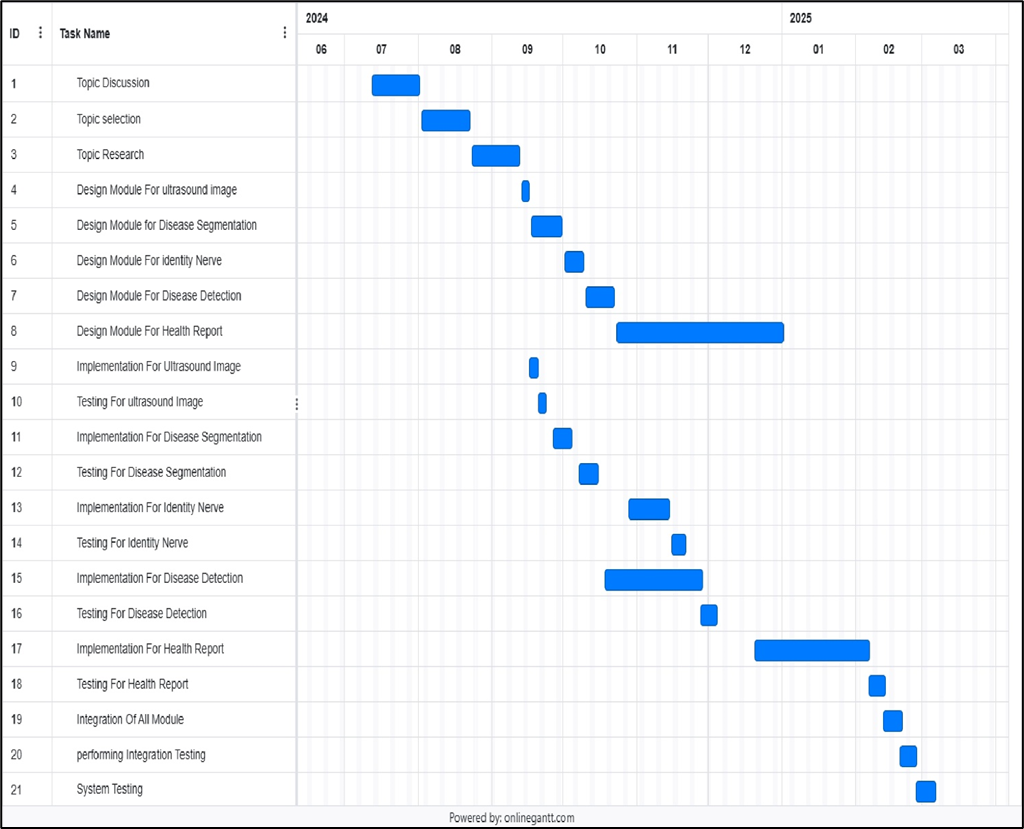
\includegraphics[width=1.05\textwidth]{image.png} % Replace with actual file
    \caption{Gantt Chart}
    \label{fig:gantt_chart}
\end{figure}

\end{document}
